\chapter{BitBucket Data Center}

\section{About BitBucket Data Center}

BitBucket Data Center is an on-premise, self-hosted SCM that is often confused with BitBucket Cloud; while there are name and some
feature similarities in both products, the integration capabilities needed by \cxoneflow
are significantly different.  This section covers configuring \cxoneflow for use with BitBucket Data Center.

The \cxoneflow endpoint \texttt{/bbdc} is the handler for all webhook event
payloads originating from BitBucket Data Center.  

\section{Webhook Topology}

\chapter{BitBucket Data Center}

\section{About BitBucket Data Center}

BitBucket Data Center is often confused with BitBucket Cloud; it should be noted that
the \cxoneflow configuration for BitBucket Data Center is not compatible with BitBucket Cloud.

\noindent\\The \cxoneflow endpoint \texttt{/bbdc} is the handler for all webhook event
payloads originating from BitBucket Data Center.  


\section{Webhook Configuration}

BitBucket Data Center can assign web hooks at the Project (aka Organization) level as well as at the
repository level.  Deploying web hook configurations for an enterprise-scale SCM is generally better
at the organization level since it will apply to all repositories in the organization.  Deploying
at the repository level is mostly suitable for testing purposes only.

Figure \ref{fig:bbdc-project-config} shows the BitBucket Data Center project configuration screen.  The
project key will appear in clone URLs and can be used as part of the regular expression 
placed in the \texttt{repo-match} configuration element.  Please see Section \ref{sec:scm-block-element} 
for a description of the \texttt{repo-match} configuration element.

The project's "Webhooks" configuration can be used to configure the \cxoneflow endpoint 
\texttt{/bbdc} to receive webhook events for each repository in the organization.  

\begin{figure}[h]
    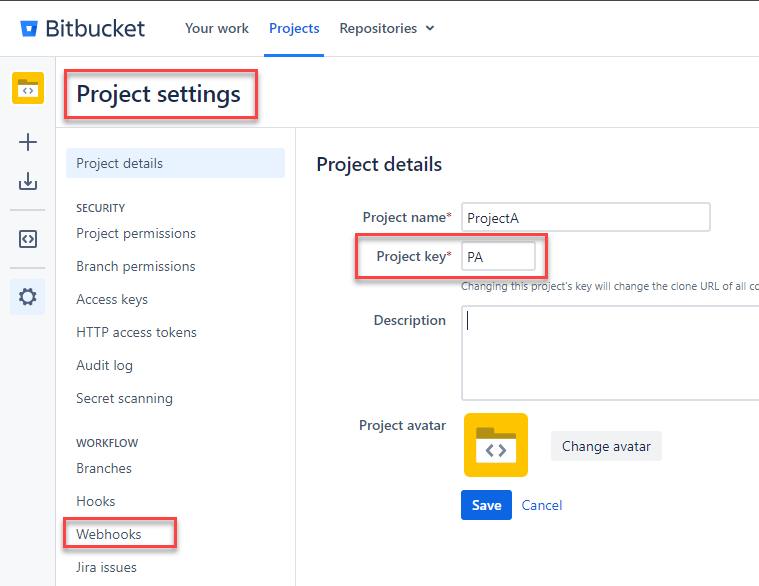
\includegraphics[width=\textwidth]{graphics/bbdc-project-config.png}
    \caption{BitBucket Data Center Project Configuration}
    \label{fig:bbdc-project-config}
\end{figure}

\begin{figure}[h]
    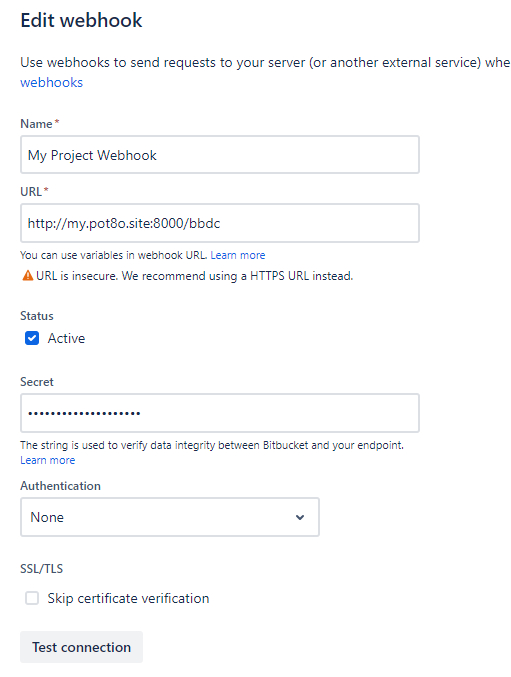
\includegraphics[width=\textwidth]{graphics/bbdc-webhook-config.png}
    \caption{BitBucket Data Center Webhook Configuration}
    \label{fig:bbdc-webhook-config}
\end{figure}



Figure \ref{fig:bbdc-webhook-config} shows a typical webhook configuration.  The Secret is how \cxoneflow
validates the origin of the event payload.  The configuration element \texttt{shared-secret}, as described
in Section \ref{sec:connection-element}, should be configured with the webhook secret value.  If \cxoneflow
is running at the specified URL endpoint, the "Test Connection" button will send a diagnostic ping
and receive back a positive response.  If the connection test fails, please ensure that \cxoneflow is running
at the address specified in the URL field and that the BitBucket Data Center server can make a connection
to that URL.

If the webhook is configured at the Project level, the events sent apply to all repositories contained
within the project.  Figure \ref{fig:bbdc-repo-event-config} shows the configured repository-level webhook 
events that will send a webhook payload to the \cxoneflow endpoint. 
Figure \ref{fig:bbdc-pr-event-config} shows the configured pull-request events that will be sent to 
the \cxoneflow endpoint.  The following events are currently supported:


\pagebreak
\begin{itemize}
    \item Repository Events
        \begin{itemize}
            \item Push
        \end{itemize}
    \item Pull Request Events
        \begin{itemize}
            \item Scanning Orchestration (Required)
                \begin{itemize}
                    \item Opened
                    \item Source branch updated
                    \item Modified
                \end{itemize}
        \end{itemize}
        \begin{itemize}
            \item Pull Request Scan Tagging (Optional)
                \begin{itemize}
                    \item Approved
                    \item Changes requested
                    \item Declined
                    \item Unapproved
                    \item Merged
                    \item Deleted
                \end{itemize}
        \end{itemize}

\end{itemize}


\begin{figure}[h]
    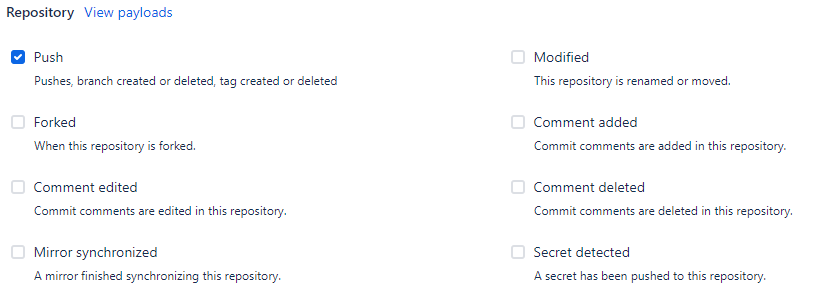
\includegraphics[width=\textwidth]{graphics/bbdc-repository-event-config.png}
    \caption{BitBucket Data Center Webhook Repository Event Config}
    \label{fig:bbdc-repo-event-config}
\end{figure}

\begin{figure}[h]
    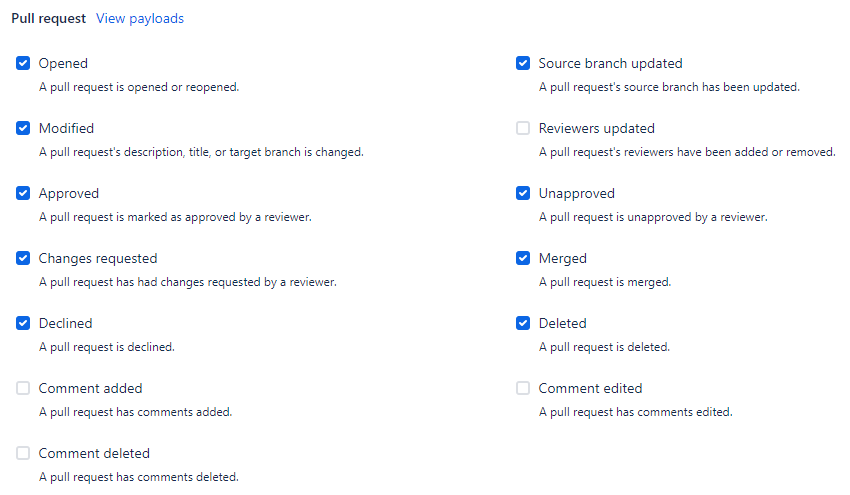
\includegraphics[width=\textwidth]{graphics/bbdc-pr-event-config.png}
    \caption{BitBucket Data Center Webhook Pull Request Event Config}
    \label{fig:bbdc-pr-event-config}
\end{figure}


\section{\cxoneflow HTTP Access Tokens}

While it is possible to use Basic Authorization to access the SCM, typically this is a configuration that
should be avoided.  The Basic Authorization is typically an interactive user account that can be subject
to password changes and Captcha verification that can break \cxoneflow operations.  It is generally
best to use a project-level HTTP Access Token for SCM connection configurations \texttt{api-auth} or
\texttt{clone-auth}.  Please refer to Section \ref{sec:connection-element} for more details about the token
configuration.

Figure \ref{fig:bbdc-token-config} shows the project-level "HTTP Access tokens" configuration.  The required
token permissions for \cxoneflow operations are:

\begin{itemize}
    \item Project read
    \item Repository read\footnote{Figure \ref{fig:bbdc-token-config} shows "Repository write".  There may be future versions of \cxoneflow that will need to create pull-request comments which will require write access.  If desired, the token can be granted "Repository read" until a write capability is released.}
\end{itemize}


\begin{figure}[h]
    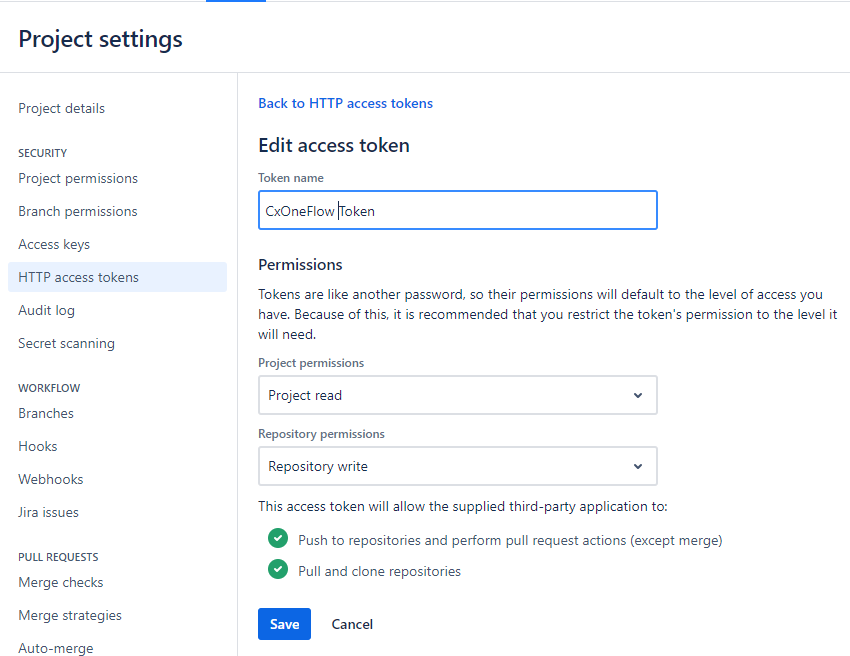
\includegraphics[width=\textwidth]{graphics/bbdc-token-config.png}
    \caption{BitBucket Data Center Project-Level HTTP Access Token Config}
    \label{fig:bbdc-token-config}
\end{figure}

Project-level access tokens do not have an associated user account.  If using project-level
access tokens, one project-level token is required per-project for which \cxoneflow is
orchestrating scans.

\section{\cxoneflow SSH Keys}

While performing scan orchestration, \cxoneflow does access the BitBucket Data Center API for
certain operations.  This requires a configuration in the \texttt{api-auth} configuration
element as described in Section \ref{sec:api-auth-element}.  The \texttt{clone-auth},
described in Section \ref{sec:clone-auth-element}, is an optional element where the credentials
used for cloning code can be provided.  If \texttt{clone-auth} is not provided, cloning will
be attempted using the credentials defined by \texttt{api-auth}.

The \texttt{clone-auth} configuration can define an SSH private key for use in cloning.  This
will allow for a separate set of credentials or authentication methods between cloning and
API use.


\section{Protected Branches}

The \cxoneflow workflow, as described in Section \ref{sec:overview}, uses the concept of "Protected Branches"
to know when to invoke workflows.  BitBucket Data Center allows for the configuration of the branching model
at the project and repository level.  Some repositories inherit their branching model from the project
configuration, but the ability for this to be overridden at the repository level is an optional configuration.
The branching model is used to determine which branches are "Protected Branches".

The project-level branching model configuration is shown in Figure \ref{fig:bbdc-branch-config}.  The
repository-level branching model configuration is similar in that both allow the definition of
"Development" and "Production" branches.  \cxoneflow considers any branch specified as a Development
or Production branch to be a "Protected Branch".

\begin{figure}[h]
    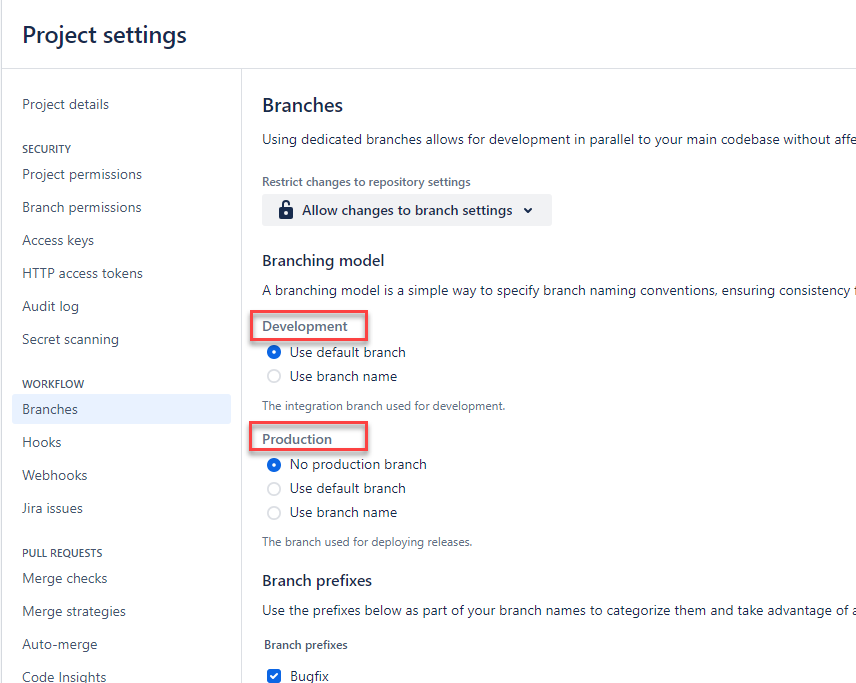
\includegraphics[width=\textwidth]{graphics/bbdc-branch-config.png}
    \caption{BitBucket Data Center Project-Level Branch Config}
    \label{fig:bbdc-branch-config}
\end{figure}



\section{Webhook Configuration}

Figure \ref{fig:bbdc-project-config} shows the BitBucket Data Center project configuration screen.  The
project key will appear in clone URLs and can be used as part of the regular expression 
placed in the \texttt{repo-match} configuration element.  Please see Section \ref{sec:yaml-config} 
for a description of the \texttt{repo-match} configuration element. The project's "Webhooks" configuration
can be used to configure the \cxoneflow endpoint \texttt{/bbdc} to receive webhook events for each repository in the organization.  

\begin{figure}[ht]
    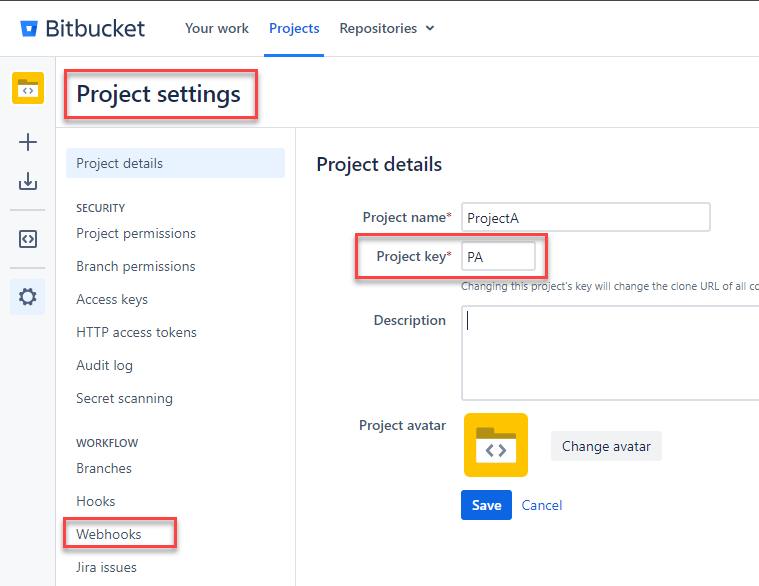
\includegraphics[width=\textwidth]{graphics/bbdc-project-config.png}
    \caption{BitBucket Data Center Project Configuration}
    \label{fig:bbdc-project-config}
\end{figure}

\begin{figure}[ht]
    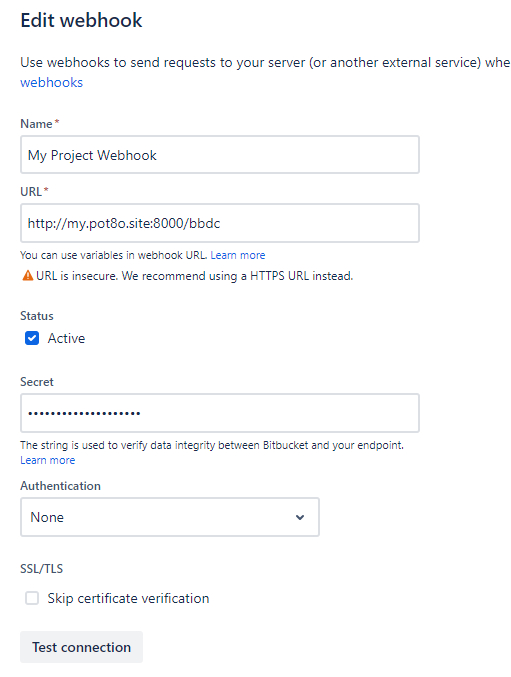
\includegraphics[width=\textwidth]{graphics/bbdc-webhook-config.png}
    \caption{BitBucket Data Center Webhook Configuration}
    \label{fig:bbdc-webhook-config}
\end{figure}


Figure \ref{fig:bbdc-webhook-config} shows a typical webhook configuration.  The \textit{Secret} is how \cxoneflow
validates the origin of the event payload.  The configuration element \texttt{shared-secret}, as described
in Section \ref{sec:yaml-config}, should be configured with the webhook secret value.  If \cxoneflow
is running at the specified URL endpoint, the "Test Connection" button will send a diagnostic ping
and receive back a positive response.  If the connection test fails, please ensure that \cxoneflow is running
at the address specified in the URL field and that the BitBucket Data Center server can make a connection
to that URL.

If the webhook is configured at the Project scope, the events sent apply to all repositories contained
within the project.  Figure \ref{fig:bbdc-repo-event-config} shows the configured repository-level webhook 
events that will send a webhook payload to the \cxoneflow endpoint. 
Figure \ref{fig:bbdc-pr-event-config} shows the configured pull-request events that will be sent to 
the \cxoneflow endpoint.  The following events are currently supported:

\begin{itemize}
    \item Repository -> Push
    \item Pull Request -> Opened
    \item Pull Request -> Source branch updated
    \item Pull Request -> Modified
    \item Pull Request -> Approved
    \item Pull Request -> Changes requested
    \item Pull Request -> Declined
    \item Pull Request -> Unapproved
    \item Pull Request -> Merged
    \item Pull Request -> Deleted
\end{itemize}


\begin{figure}[ht]
    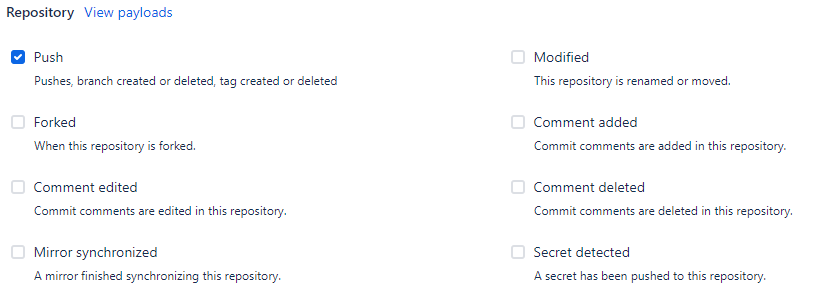
\includegraphics[width=\textwidth]{graphics/bbdc-repository-event-config.png}
    \caption{BitBucket Data Center Webhook Repository Event Config}
    \label{fig:bbdc-repo-event-config}
\end{figure}

\begin{figure}[ht]
    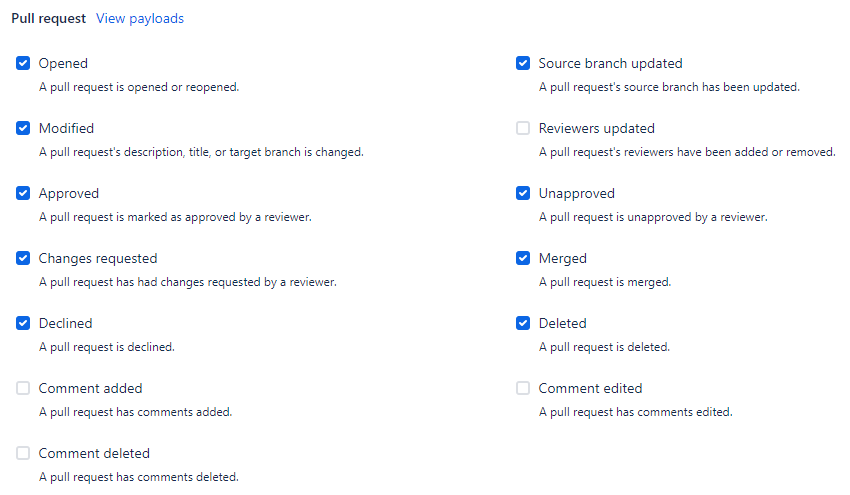
\includegraphics[width=\textwidth]{graphics/bbdc-pr-event-config.png}
    \caption{BitBucket Data Center Webhook Pull Request Event Config}
    \label{fig:bbdc-pr-event-config}
\end{figure}


\section{\cxoneflowtext\space HTTP Access Tokens}

Current versions of BitBucket Data Center now reject the use of Basic Authorization using
a username and password. While it may be possible to use Basic Authorization to access the SCM, typically
this is a configuration that should be avoided.  In addition to Basic Authorization breaking upon BitBucket Data Center
server upgrades, an interactive user account may be subject to password changes and Captcha verification that
can break \cxoneflow operations.  

It is generally best to utilize a user HTTP access token for SCM connection
configurations \texttt{api-auth}.  If a user HTTP access token is used, the user can be granted
permissions for multiple projects; this will make the \cxoneflow configuration much easier. 

BitBucket Data Center can create project HTTP access tokens that are similar in use to
a user HTTP access token.  A project HTTP access token is not tied to a specific user, but the
access scope is limited to accessing repositories in the project where it was generated.
If using project HTTP access tokens, one project HTTP access token is required for \cxoneflow
to handle events emitted from repositories in each corresponding project. This also implies that
the \cxoneflow configuration will require one SCM service configuration per project with an
associated \texttt{repo-match} regular expression so the correct project token is used when
orchestrating the scan.

Please refer to Section \ref{sec:yaml-config} for more details about using the HTTP access token
to configure the BitBucket Data Center connection.

Figure \ref{fig:bbdc-token-config} shows the project "HTTP Access tokens" configuration.  The required
token permissions for \cxoneflow operations for any HTTP access token are:

\begin{itemize}
    \item Project read
    \item Repository read
    \item Repository write
\end{itemize}


\begin{figure}[ht]
    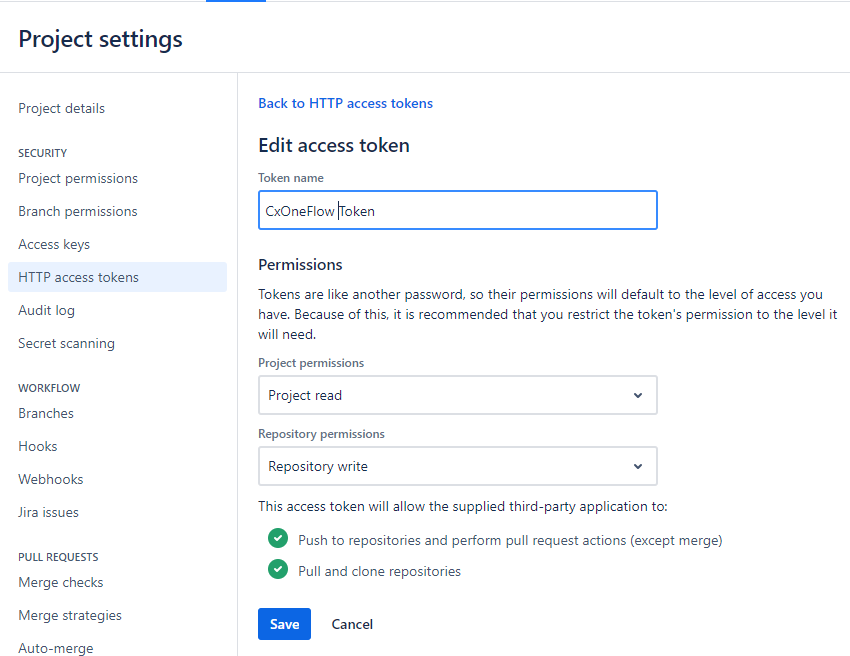
\includegraphics[width=\textwidth]{graphics/bbdc-token-config.png}
    \caption{BitBucket Data Center Project-Level HTTP Access Token Config}
    \label{fig:bbdc-token-config}
\end{figure}


User HTTP access tokens are tied to a user account but are not subject to password
changes, 2FA authentication, and captcha challenges with interactive logins.  A token generated
from a user as a service account can be granted the required permissions across multiple projects.
In this scenario, a single SCM service configuration would be able to handle events coming from
repositories in multiple projects.

\section{\cxoneflowtext\space SSH Keys}

While performing scan orchestration, \cxoneflow does access the BitBucket Data Center API for
certain operations.  This requires a configuration in the \texttt{api-auth} configuration
element as described in Section \ref{sec:yaml-config}.  The \texttt{clone-auth},
described in Section \ref{sec:yaml-config}, is an optional element where the credentials
used for cloning code can be provided.  If \texttt{clone-auth} is not provided, cloning will
be attempted using the credentials defined by \texttt{api-auth}.

The \texttt{clone-auth} configuration can define an SSH private key for use in cloning.  This
will allow for a separate set of credentials or authentication methods between cloning and
API use.


\section{Protected Branches}

The \cxoneflow workflow, as described in Section \ref{sec:overview}, uses the concept of "Protected Branches"
to know when to invoke workflows.  BitBucket Data Center allows for the configuration of the branching model
at the project and repository level.  Some repositories inherit their branching model from the project
configuration, but the ability for this to be overridden at the repository level is an optional configuration.
The branching model applied to the repository that emitted the webhook event is used to determine which branches
are "Protected Branches" at the time \cxoneflow handles the event.

The project-level branching model configuration is shown in Figure \ref{fig:bbdc-branch-config}.  The
repository-level branching model configuration is similar in that both allow the definition of
"Development" and "Production" branches.  \cxoneflow considers any branch specified as a Development
or Production branch to be a "Protected Branch".

\begin{figure}[ht]
    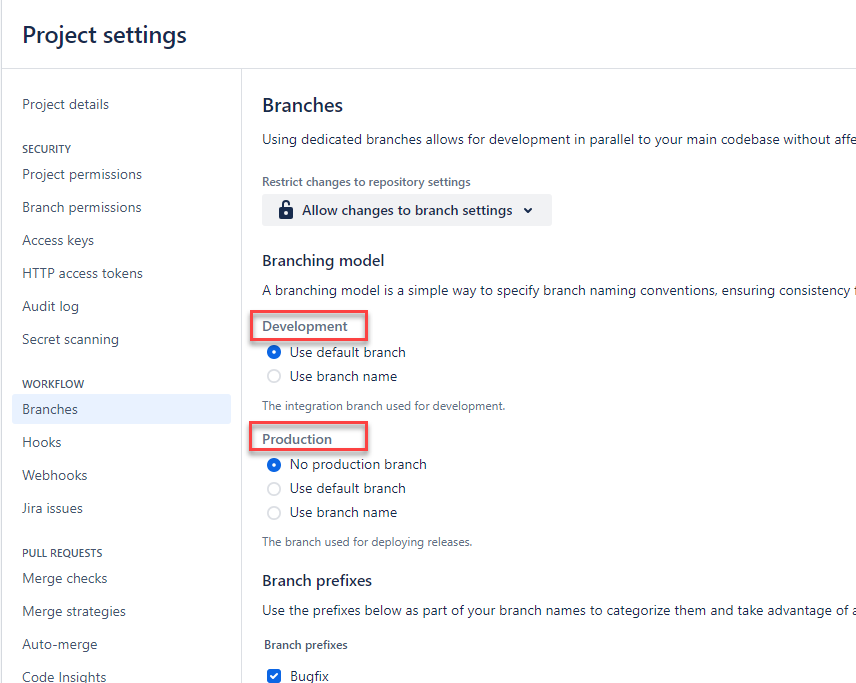
\includegraphics[width=\textwidth]{graphics/bbdc-branch-config.png}
    \caption{BitBucket Data Center Project-Level Branch Config}
    \label{fig:bbdc-branch-config}
\end{figure}

